\documentclass[pageno]{jpaper}

\usepackage[normalem]{ulem}

% Packages
\usepackage{epstopdf}
\usepackage{mathtools}
\DeclarePairedDelimiter{\ceil}{\lceil}{\rceil}
\DeclarePairedDelimiter{\floor}{\lfloor}{\rfloor}

\begin{document}

\title{NeuroCube: Low-Power Scalable Neuromorphic Architecture Using Hybrid Memory Cube}


\date{}
\maketitle

\thispagestyle{empty}

\begin{abstract}
This document serves as a sample for submissions to MICRO 2014.
We provide some guidelines that authors should follow when submitting papers to
the conference.
\end{abstract}

\section{Introduction}\label{sec:Introduction}

THIS PART IS FOR INTRODUCTION

1. Machine Learning is important application in RMS (Recognition/Mining/Synthesis)

2. Since its application scope increases and handle the big data, input domain and complexity increases dramatically

3. NN is one of the well known algorithms for ML, and large scale of NN is required to solve complex ML problem.

4. Large scale NN means more neurons, more layers, and more weight. Therefore, it requires massive computations and data storage

5. For given hardware, there are two methods to solve this problem.

5-1. First method is algorithm multiplexing, which divides the problem into sub-problems, and conquer them. It's hardware overhead/requirement is low, but it can't solve the problem requiring global optimization, for example, hole filling.

5-2. Another method, which we adapt, storing all neural network in 'external' memory, which can have high capacity with long latency and share some computational units in given hardware.

6. Interesting part is that operation of neural network is determined by data access sequence of memory since most of digital NNs are based on similar operations such as multiply-and-accumulate or sigmoid function. Therefore changing the data access sequency can implements different neural networks with given hardware.

7. Since entire neural network is stored in memory, accessing memory is the key operation in neural network. 

8. Based on given neural network, data sequence is not random sequence, but it is predetermined by algorithm. Therefore, dedicated memory controller generating data request and address can be implemented for each neural entwork. This controller is the key element for neural network function. 

9. This controller will make memory deliver the data to multiple processing engines without request to operate multiple PEs in parallel without stall due to memory access (full utilization).

10. For the application requiring sharing the data between PEs, network-on-chip is required to connect multiple PEs and multiple Memory. As data sequence is determined by neural network type, network traffic is also determined by neural network.

11. In this paper, we will investigate architecture for digital neuromorphic hardware including multiple processing engines, cache memory, network-on-chip, external memory, and memory controller.

12. Under the given external memory and processing engines, optimal number of cache memory and processing engines  will be studied to maintail full utilization of PEs.

13. For different NNs, memory controller is implemented, and its perforamnce will be analyzed for different applications. 

14. With given architecture, network traffic pattern on NoC will be studied and performance of entier system will be discussed.

15. To achieve high external memory bandwidth, hybrid memory cube could be appropriate system for neuromorphic architecture. Its advantage will be analyzed for different NNs.


%This document provides the formatting instructions for submissions to the 47th
%Annual IEEE/ACM International Symposium on Microarchitecture,
%2014~\cite{micro47}. In an effort to respect the efforts of reviewers and in
%the interest of fairness to all prospective authors, we request that all
%submissions to MICRO-47 follow the formatting and submission rules detailed
%below.  Submissions that (grossly) violate these instructions may not be
%reviewed, at the discretion of the program chair, in order to maintain a review
%process that is fair to all potential authors.
%
%An example submission (formatted using the MICRO-47 submission format) that
%contains the submission and formatting guidelines can be downloaded from here:
%\href{http://www.microarch.org/micro47/files/micro47-template.pdf}{Sample
%PDF}. The contents of this document are the same as the contents of the
%submission instructions that appear on
%\href{http://www.microarch.org/micro47/submission.html}{this website}.
%
%All questions regarding paper formatting and submission should be directed to
%the program chair.

\section{Previous Work}\label{sec:Previous works}
In this section, we will introduce recent machine learning techniques using different types of neural network and hardware implementation based on ASIC or FPGA. 

\subsection{Neural network for machine learning} \label{sub_sec:Previous works algorithm}
Artificial Neural network (neural network) which mimics biological neural networks is the most interested topic in machine learning. It is composed of set of neurons and a single neuron may connect to set of other neuron or all neurons in the network. This network could be composed of multiple layers --> Deep NN?

% How can we classify different NNs.
Main benefits of Neural network are the characteristic of computation process in biological neural network, such as parallelism, nonlinearity, error-robustness, and learning (plasticity). Therefore neural networks can be classified based on these different characteristics \cite{basheer2000artificial}. According to Section 6 in \cite{basheer2000artificial}, neural network can be classified based on different characteristics such as target application, connectivity, flow of network. In terms of hardware design for neural network, we should note that connectivity and flow of network are most important factors of neural network since these factors are directly related to the interface in the system (for example, bus-interface or network-on-chip (NoC)). 

\textbf{Connectivity}

A single neuron can connect with all neurons in the network or set of neurons. Hopfiled network is the network with fully connected two layers \cite{hopfield1984neurons}. Full connectivity means outputs of all neurons (including itself) are fed into as input to a single neuron. Due to its complexity of network, it is impractical to implement in real hardware. 
% Is there any benefit in Hopfield Network thanks to fully connection?

In stead of fully connection, cellular neural network has local connection; a single neuron connects to the set of neurons in the neighborhood \cite{chua1988cellular}. A single neuron is connected with \begin{math} (2r+1)^2 \end{math} neurons when radius of neighborhood is \begin{math}r\end{math}. For simple image processing (such as edge detection\cite{chua2002cellular}, garbor filter \cite{egmont2002image}), \begin{math} r=1\end{math} is enough and \begin{math} r=3\end{math} is still enough for associative memory operation (reference is required).

\textbf{Network flow}




1. Why do we need different NNs other than Convolution NNs? --> Deep learning requires `different' type of neural network layers

2. What is the characteristic of diff. NNs (pro - cons) or appropriate application

Can we compute number of basic computations such as multiplications or additions for some applications? 

Maybe table to compare diff NNs will be good.

\subsection{Algorithm multiplexing} \label{sub_sec:alg_mux}
Describe algorithm multiplexing

\subsection{Hardware sharing?} \label{sub_sec:hw_share}
Describe hardware sharing and compare with algorithm multiplexing

\subsection{Neuromorphic hardware implementation}\label{sub_sec:Previous works hardware}
Following hardware sharing



\begin{figure}[!t]
\centering
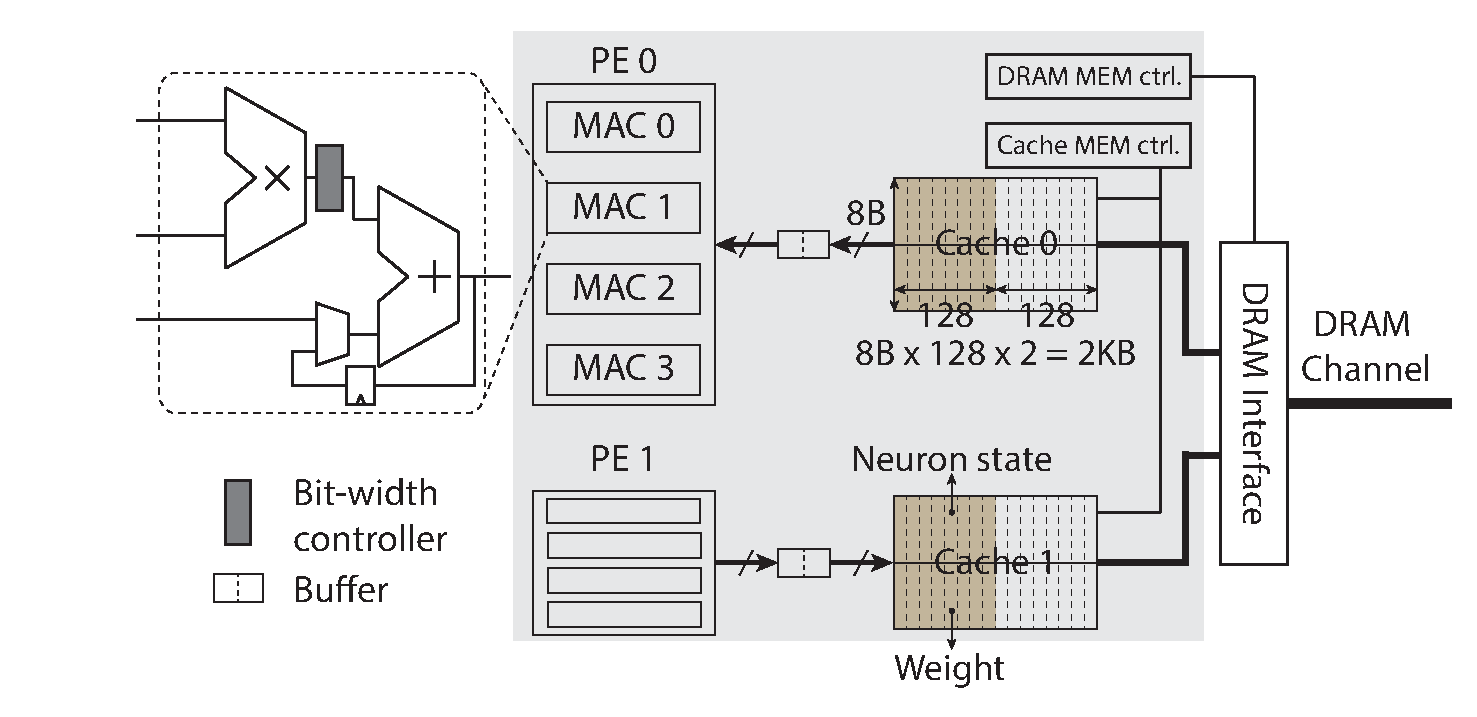
\includegraphics[width=3.5in]{fig/Full_system_MLP_ver2.eps}
\caption{Full system MLP ver2 from 15-DAC.}
\label{fig:MLP_system}
\end{figure}


\section{Reconfigurable Neuromorphic Architecture}\label{sec:architecture}
text
\subsection{External memory}\label{sub_sec:ext_mem}
text
\subsection{Cache memory}\label{sub_sec:cache_mem}
cache memory

\subsection{Processing elements}\label{sub_sec:pe}
As we explained before, main basic operations for NNs are multiplication, addition, activation function, sampling ... So we will prepare all functions to cover different neural networks. Then controlling the data from memory to processing elements can implement different neural networks.
\subsection{Network-on-chip}\label{sub_sec:noc}
text

\subsection{Memory architecture}\label{sub_sec:mem_arch}
As stated in Section \ref{sub_sec:Previous works hardware}, we design the digital MLP hardware fully utilizing MAC units. To make the MLP hardware scalable to larger network size, the on-chip cache memories should interface with an external DRAM memory (Fig.~\ref{fig:MLP_system}). However, the DRAM access latency sacrifices the parallelism provided by MLP algorithm. We have to choose the maximum number of MAC units in each PE at design time depending on the memory architecture to achieve full utilization.
To begin with, the read latency of DRAM can be defined as (MLP operation is read-intensive, thus, we focus on the read latency):

%DRAM_{lat} = tRCD + tCAS + tRP + \floor[\bigg]{\frac{\left(\frac{page\_size}{bit\_width_{bus}}-1\right)}{2}},
\begin{equation}
	DRAM_{lat} = tRCD + tCAS + tRP + \floor[\bigg]{\left(\frac{page\_size}{bit\_width_{bus}}-1\right)/2},
	\label{eq:DRAM_LAT}
\end{equation}

where $tRCD$ is the number of clocks required to access each row, $tCAS$ is the column access latency, and $tRP$ is the required clocks between row precharge and activate. Each parameter in (\ref{eq:DRAM_LAT}) is determined by the specification of the external memory. Also, we assume that the burst length can be modified to read the whole page after a single row access (since MLP has a memory access pattern with strong spatial coherence) with low column access latency. Let’s consider we have an external memory which can be accessed at $f_{DRAM}$ (= $1/CLK_{DRAM}$). Here, $CLK_{DRAM}$ represents the DRAM I/O bus clock cycle. We then choose PE to operate at $f_{PE}$ and SRAM memories to operate at $f_{SRAM}$. Then, $DRAM_{lat}$ can be rewritten by using $f_{PE}$.

\begin{equation}
	DRAM_{lat\-PE} = DRAM_{lat} \times \frac{f_{PE}}{f_{DRAM}}.
	\label{eq:DRAM_LAT_PE}
\end{equation}

As shown in Fig.~\ref{fig:MLP_system}, the half of the cache (equivalent to the page size of DRAM) has to be initially filled up to fetch in the data into each PE (a group of MAC units) in parallel. The 8Byte is the data size required at each MAC unit for matrix-vector multiplication. After initialization, each cache is updated with round-robin scheduling in parallel with the data read from the cache to PE (Fig.~\ref{fig:MLP_system}). To achieve the full utilization, the following condition has to be satisfied.

\begin{equation}
	\frac{\#Lines}{m}=DRAM_{lat\-PE}\times n,
	\label{eq:num_lines_per_PE}
\end{equation}

where m is the number of MAC units in a PE, n is the number of PEs, and \#Lines is the (page\_size/word\_size). The left-hand side of (\ref{eq:num_lines_per_PE}) defines the clock cycles to use all data stored in the half portion (shaded) of the cache. The right-hand side of (\ref{eq:num_lines_per_PE}) represents the clock cycles to prepare data for all PEs connected to each channel (filling up the other half).\textit{ Equation (\ref{eq:num_lines_per_PE}) determines the total number of MAC units \begin{math}(n\times m)\end{math} that can be designed without sacrificing the full utilization.} The question then arises how to set the number of MAC units per PE (= $‘m’$). This is determined by the clock frequency ratio between the cache and the PE ($f_{SRAM}/ f_{PE}$). At each $CLK_{SRAM}$, the cache provides 8B data to the buffer. This may be continued for $k\times CLK_{SRAM}$, which allows total 8kB for a PE to use at one $CLK_{PE}$ (If the frequency ratio is 4, then the data size the cache can provide within one $CLK_{PE}$ becomes 32B). Thus, the number of MAC units per PE is constrained by

\begin{equation}
	m=\frac{f_{SRAM}}{f_{PE}}=\frac{CLK_{PE}}{CLK_{SRAM}},
	\label{eq:num_m}
\end{equation}

This relation naturally leads to the decision of the number of PEs, $n$. Since the total number of MAC units is determined by (\ref{eq:num_lines_per_PE}), sets of $(m, n)$ can be obtained. Here, as reducing the number of cache memories results in smaller area and lower power, selecting smaller $n$ is a better design option with a given memory architecture. This is for one channel case so the total number of MAC units $(NUM_{MAC})$ with multi-channel memory becomes:

\begin{equation}
	NUM_{MAC}=\#Channel\times(n\times m).
	\label{eq:num_mac}
\end{equation}











\section{Traffic Analysis on Network-on-Chip}
For different neural networks, our system described in previous sesction is simulated to operate given testcase for each neural network. For this system, standard DDR3-SDRAM (low bandwidth specification) is assumed as external DRAM.




\section{Hybrid Memory Cube}
hmc introduce
\subsection{Architecture of HMC}
hmc introduce
\subsection{Intranetwork of HMC through logic die}
hmc introduce
\subsection{Internetwork of HMC through high speed links}
hmc introduce
\subsection{Neurocube using Intranetwork of HMC}
Processor-in-Memory (PIM) design hmc introduce
Area/power/thermal limitation

\section{Traffic Analysis of NeuroCube}
Introduce improvement of NeuroCube with HMC with high bandwidth


\section{Conclusions}
conclusions 
bla bla bla \cite{basheer2000artificial}.


%%% MICRO: Max 11 Pages without Reference. There is no limit for Reference
\clearpage
\bstctlcite{bstctl:etal, bstctl:nodash, bstctl:simpurl}
\bibliographystyle{IEEEtranS}
\bibliography{references}

\end{document}




%%% FIGURE
%\begin{figure}[!t]
%\centering\includegraphics[width=4.8in]{figs/tm_pl_orig.pdf}
%\caption{Setup and hold time constraints of pulsed latch circuits.}
%\label{fig: timing_pl_orig}
%\end{figure}



%%%%%%%%%%%%%  MICRO TEMPLATE %%%%%%%%%%%%%%%%%
%For MICRO-47, we are instituting a new paper submission format
%and reference requirements. All submissions are allowed a maximum 
%of 11 pages of single-spaced two-column text content according to
%the formatting guidelines below.  In addition, submissions are 
%allowed a references section of unlimited length outside of this
%11-page limit.  

%References must include complete author lists to facilitate
%the reviewing process.	





%If you are using \LaTeX~to typeset your paper, then we suggest
%that you use the template available here:
%\href{http://www.microarch.org/micro47/files/micro47-latex-template.tar.gz}{\LaTeX~Template}.
%(\href{http://www.microarch.org/micro47/files/micro47-template.pdf}{This
%document} was prepared with that template.)  If you are using a different
%software package to typeset your paper, then please adhere to the guidelines
%mentioned in Table~\ref{table:formatting}.
%
%\begin{table}[h!]
%  \centering
%  \begin{tabular}{|l|l|}
%    \hline
%    \textbf{Field} & \textbf{Value}\\
%    \hline
%    \hline
%    Page limit & 11 pages + references\\
%    \hline
%    Paper size & US Letter 8.5in $\times$ 11in\\
%    \hline
%    Top margin & 1in\\
%    \hline
%    Bottom margin & 1in\\
%    \hline
%    Left margin & 0.75in\\
%    \hline
%    Right margin & 0.75in\\
%    \hline
%    Space between columns & 0.25in\\
%    \hline
%    Body font & 10pt\\
%    \hline
%    Abstract font & 10pt, italicized\\
%    \hline
%    Section heading font & 12pt, bold\\
%    \hline
%    Subsection heading font & 10pt, bold\\
%    \hline
%    Caption font & 9pt, bold\\
%    \hline
%    References & 8pt, no page limit, list all authors\\
%    \hline
%  \end{tabular}
%  \caption{Formatting guidelines for submission.}
%  \label{table:formatting}
%\end{table}

%\textbf{Please ensure that you include page numbers with your
%submission}. This makes it easier for the reviewers to refer to
%different parts of your paper when they provide comments.


%
%\noindent\textbf{\sout{Author List.}} All submissions are double
%blind. Therefore, please do not include any author names in the
%submission. You must also ensure that the metadata included in the
%PDF does not give away the authors. If you are improving upon your
%prior work, refer to your prior work as a third person and include
%references to your past work. 
%
%\noindent\textbf{Figures and Tables.} Ensure that the figures and
%tables are legible.  Please also ensure that you refer to your
%figures in the main text. Many reviewers print the papers in
%gray-scale. Therefore, if you use colors for your figures, ensure
%that the different colors are distinguishable in gray-scale.
%
%\noindent\textbf{Main Body.} Avoid bad page or column breaks in
%your main text, i.e., last line of a paragraph at the top of a
%column or first line of a paragraph at the end of a column. If you
%begin a new section or sub-section near the end of a column,
%ensure that you have at least 2 lines of body text on the same
%column. Note that the entire main body of your submission as well as any
%Figures, footnotes, etc., must conform to the 11-page content limit;
%only references may appear on additional pages.
%
%\noindent\textbf{References.} There is no length limit for references. 
%Each reference must explicitly list all authors of the paper. 
%Papers not meeting this requirement will be rejected. Authors of NSF 
%proposals should be familiar with this requirement. Knowing all
%authors of related work will help find the best reviewers.
%
%\section{Submission Instructions}
%
%\subsection{Paper Authors}
%
%Declare all the authors of the paper upfront. Addition/removal of authors once
%the paper is accepted will have to be approved by the program chair.
%
%\subsection{Conflict Responsibilities}
%
%Authors must register all their conflicts on the paper submission site. 
%Conflicts are needed to ensure appropriate assignment of reviewers. If a paper
%is found to have an undeclared conflict that causes a problem OR if a paper 
%is found to declare false conflicts in order to abuse or "game" the review 
%system, the paper may be rejected. 
% 
%Please declare a conflict of interest (COI) with the following for any author of your paper:
%
%\begin{enumerate}
%\item Your Ph.D. advisor, post-doctoral advisor, and Ph.D. students
%\item Other past or current advisors
%\item Current or past students
%\item Family relations by blood or marriage (if they might be potential reviewers)
%\item People with the same affiliation
%\item People whom you co-authored accepted/rejected/pending papers with in the last 5 years
%\item People whom you co-authored accepted/pending grant proposals with in the last 5 years
%\end{enumerate}
%
%"Service" collaborations like co-authoring a CSTB report or co-presenting tutorials do 
%not constitute conflicts. However, there may be others not covered 
%by the above with whom you know a COI exists. Please report such COIs; however, you 
%will need to justify them. Please be reasonable. For example, just because a reviewer
%works on similar topics as your paper, you cannot declare a COI with that reviewer. We
%will carefully check the justification of conflicts and take action when authors seem to be 
%blacklisting reviewers without sufficient justification. 
%
%We hope to draw most reviewers 
%from the PC and the ERC, but others from the community may also write reviews. Please
%declare all your conflicts (not just restricted to the PC and ERC). When in doubt, 
%contact the program chair.
%
%
%\subsection{Concurrent Submissions and Resubmissions of Already Published Papers}
%
%By submitting a manuscript to MICRO-47, the authors guarantee that the
%manuscript has not been previously published or accepted for
%publication in a substantially similar form in any conference or
%journal. The authors also guarantee that no paper which contains
%significant overlap with the contributions of the submitted paper is
%under review to any other conference or journal or workshop, or will
%be submitted to one of them during the MICRO-47 review
%period. Violation of any of these conditions will lead to rejection.
%
%Extended versions of papers accepted to IEEE Computer Architecture
%Letters can be submitted to MICRO-47.
%As always, if you are in doubt, it is best to contact the program chair. 
%
%\section{Submission Site}
%
%A link to the submission site will be posted on the MICRO-47 web site
%\href{http://www.microarch.org/micro47/}{http://www.microarch.org/micro47/}
%in mid April. 



